%%%%%%%%%%%%%%%%%%%%%%%%%%%%%%%%%%%%%%%%%%%%%%%%%%%%%%%%%%%%%%%%%%%%%%%%%%%%%%%
% Chapter 3: Resultados
%%%%%%%%%%%%%%%%%%%%%%%%%%%%%%%%%%%%%%%%%%%%%%%%%%%%%%%%%%%%%%%%%%%%%%%%%%%%%%%

%++++++++++++++++++++++++++++++++++++++++++++++++++++++++++++++++++++++++++++++

Finalizada la etapa de desarrollo del Trabajo de Fin de Máster, se procede a describir la herramienta implementada.
\bigskip

La herramienta se ha denominado {\bfseries \verb|ghhell|}, abreviatura de {\it GitHub Shell}. Se ha publicado en NPM\cite{URL:NPM} para su fácil distribución e instalación:
\bigskip

\begin{figure}[H]
\begin{center}
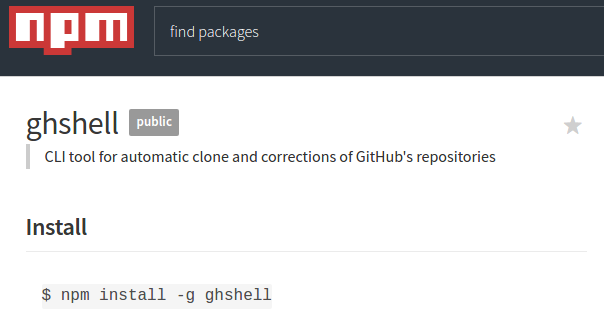
\includegraphics[width=0.8\textwidth]{images/npm1}
\caption{Página del gestor de paquetes NPM}
\label{fig:npm}
\end{center}
\end{figure}

Las funcionalidades implementadas en \verb|ghshell|, se describen a continuación. 
\bigskip

{\bfseries NOTA}: se puede consultar toda la información detallada referente a los comandos del programa en el Apéndice \ref{subsec:b.2.2}.

%---------------------------------------------------------------------------------
\section{Funcionalidades requeridas}
\label{3:sec:1}

%------------------------------------------------------------------------------------------------------------
\subsection{Autenticación con GitHub}
\label{subsec:3.1.1}
    
    Una vez que el usuario se autentifica con GitHub, se genera un \ceit{\ref{apend1:token}} personal, que se usa posteriormente para acceder a la \ceit{\ref{apend1:api}} de Github. 
\bigskip
   
   Este token se almacena cifrado en el equipo del usuario, por lo que las siguientes ocasiones que utilice la herramienta no hará falta que vuelva a iniciar sesión:
        
        \begin{figure}[H]
		\begin{center}
		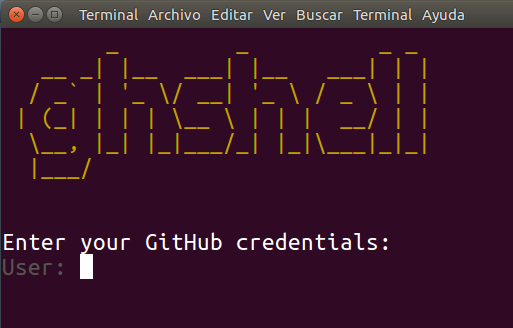
\includegraphics[width=0.7\textwidth]{images/ghshell1}
		\caption{Login de usuario}
		\label{fig:ghshell1}
		\end{center}
		\end{figure}
		
		\begin{figure}[H]
		\begin{center}
		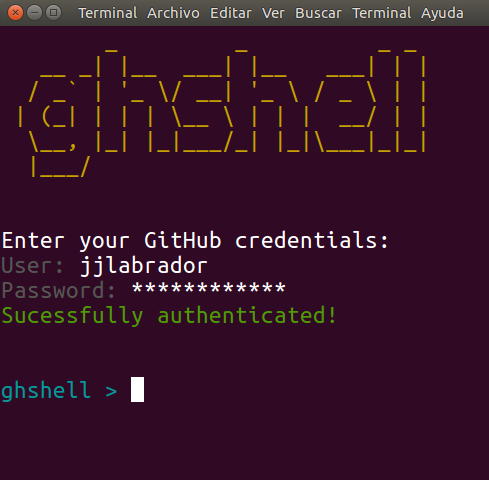
\includegraphics[width=0.6\textwidth]{images/ghshell2-1}
		\caption{Usuario autenticado}
		\label{fig:ghshell2-1}
		\end{center}
		\end{figure}
		
		\begin{figure}[H]
		\begin{center}
		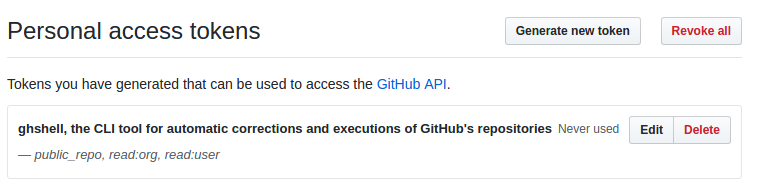
\includegraphics[width=1\textwidth]{images/ghshell2-3}
		\caption{Token personal en GitHub}
		\label{fig:ghshell2-3}
		\end{center}
		\end{figure}
		
		\begin{figure}[H]
		\begin{center}
		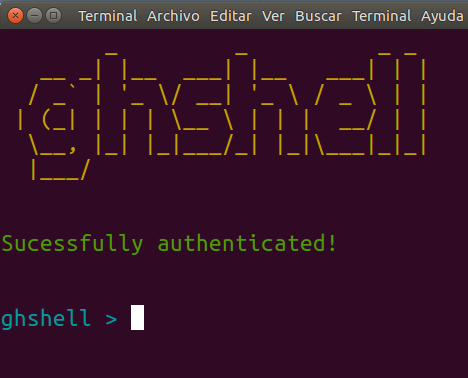
\includegraphics[width=0.6\textwidth]{images/ghshell2-4}
		\caption{Login automático una vez generado el token}
		\label{fig:ghshell2-4}
		\end{center}
		\end{figure}
		
	Si el usuario cierra sesión en la herramienta, se eliminará el token en GitHub y en el equipo:
	
		\begin{figure}[H]
		\begin{center}
		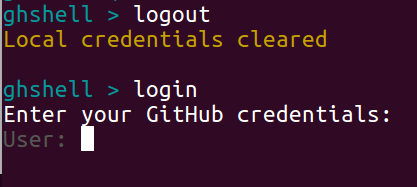
\includegraphics[width=0.6\textwidth]{images/ghshell2-2}
		\caption{Logout de usuario}
		\label{fig:ghshell2-2}
		\end{center}
		\end{figure}

\newpage
%------------------------------------------------------------------------------------------------------------
\subsection{Listar organizaciones, asignaciones y repositorios de GitHub del usuario}
\label{subsec:3.1.2}   
    
    Con el comando \verb|orgs -l|, se puede listar las organizaciones del usuario y usando \verb|repos -l|, se listarán los repositorios del usuario. 
\bigskip
    
    Se puede acceder 'virtualmente' a las organizaciones y listar los repositorios que contiene, así como las asignaciones.
\bigskip
            
        \begin{figure}[H]
		\begin{center}
		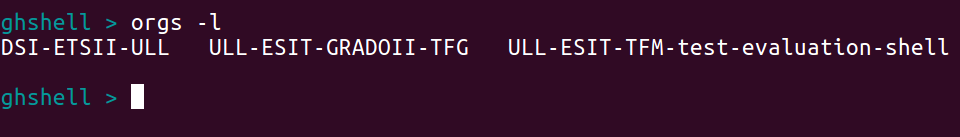
\includegraphics[width=0.9\textwidth]{images/ghshell3}
		\caption{Lista de organizaciones del usuario}
		\label{fig:ghshell3}
		\end{center}
		\end{figure}
		
		\begin{figure}[H]
		\begin{center}
		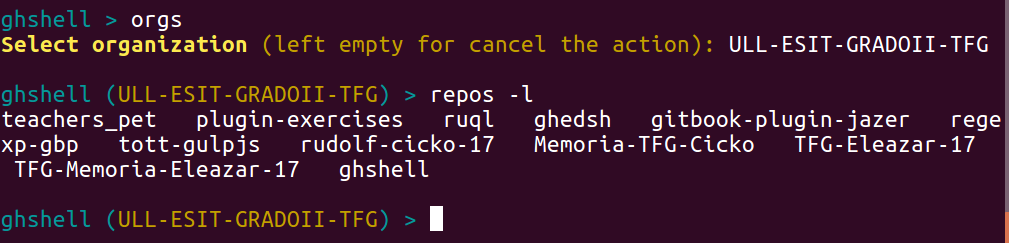
\includegraphics[width=0.9\textwidth]{images/ghshell4}
		\caption{Lista de repositorios de una organización}
		\label{fig:ghshell4}
		\end{center}
		\end{figure}
		
		\begin{figure}[H]
		\begin{center}
		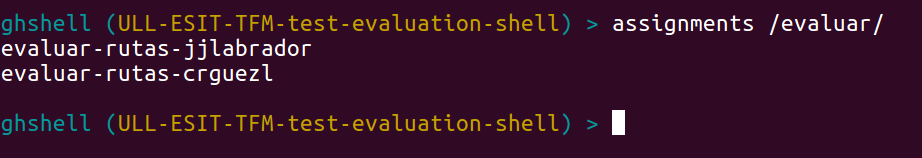
\includegraphics[width=0.9\textwidth]{images/ghshell5}
		\caption{Asignaciones dentro de otra organización}
		\label{fig:ghshell5}
		\end{center}
		\end{figure}

\newpage

	También es posible acceder 'virtualmente' a los repositorios dentro una organización y realizar acciones sobre ellos:
	
		\begin{figure}[H]
		\begin{center}
		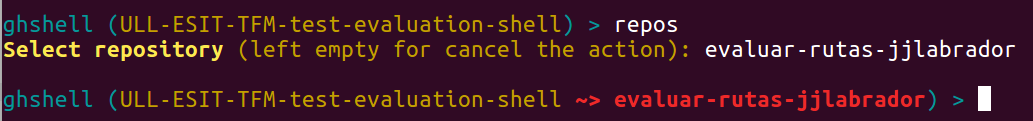
\includegraphics[width=1\textwidth]{images/ghshell5-1}
		\caption{Acceso a un repositorio de una organización}
		\label{fig:ghshell5-1}
		\end{center}
		\end{figure}

%------------------------------------------------------------------------------------------------------------
\subsection{Automatizar la descarga de repositorios}
\label{subsec:3.1.3}  
        	
    En función del contexto dónde nos encontremos dentro de la herramienta, podremos:
    \begin{itemize}
    	\item Clonar el repositorio en el que nos encontremos.
    	\item Clonar un repositorio determinado.
	    \item Clonar todos los repositorios que coincidan con una determinada expresión regular.
	    \item Clonar todos los repositorios de una asignación que coincidan con una determinada expresión.
    \end{itemize}
    
    El clonado se realiza de manera \ceit{\ref{apend1:asincrona}}, por lo que podemos seguir trabajando mientras se clona(n) el/los repositorio(s). 
\bigskip
   
   Se puede observar el estado de la clonación revisando el fichero de log que se genera cuyo nombre sigue el formato: \textless \verb|nombre-repositorio|\textgreater \verb|-clone.log|.
    
    	\begin{figure}[H]
		\begin{center}
		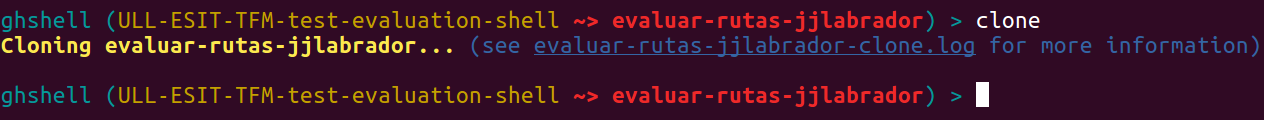
\includegraphics[width=1\textwidth]{images/ghshell6-3}
		\caption{Clonado del repositorio donde nos encontramos}
		\label{fig:ghshell6-3}
		\end{center}
		\end{figure}	

\newpage

    Si clonamos repositorios que pertenecen a una organización, se creará una carpeta con el nombre de la organización y en su interior se guardarán los repositorios clonados.
    		
	Además, si clonamos repositorios que pertenecen a una asignación, también se creará una carpeta con el nombre de la asignación que los contendrá.
	
        \begin{figure}[H]
		\begin{center}
		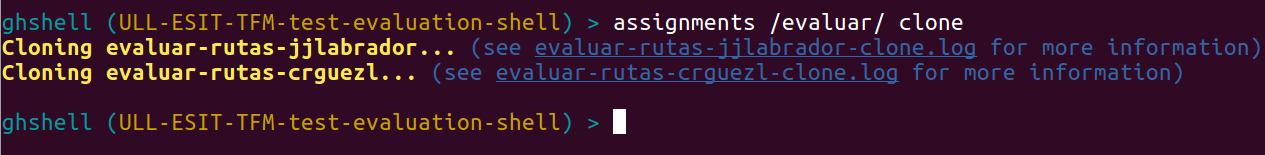
\includegraphics[width=1\textwidth]{images/ghshell6-1}
		\caption{Clonado de asignaciones que coinciden con una expresión regular}
		\label{fig:ghshell6-1}
		\end{center}
		\end{figure}	
		
		\begin{figure}[H]
		\begin{center}
		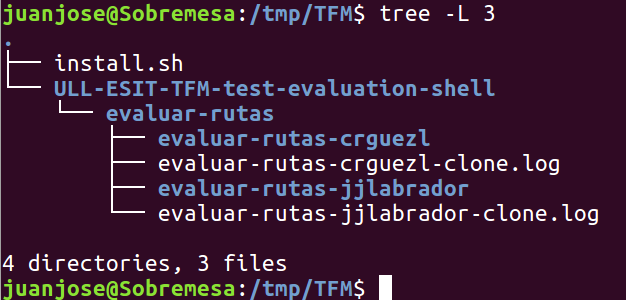
\includegraphics[width=0.7\textwidth]{images/ghshell6-2}
		\caption{Resultado del clonado}
		\label{fig:ghshell6-2}
		\end{center}
		\end{figure}

\newpage
%------------------------------------------------------------------------------------------------------------
\subsection{Automatizar la ejecución de scripts en los repositorios}
\label{subsec:3.1.3} 
	    
    En función del contexto donde nos encontremos dentro de la herramienta, podremos:
    \begin{itemize}
    	\item Ejecutar un script en el repositorio en el que nos encontremos.
    	\item Ejecutar un script en un determinado repositorio.
	    \item Ejecutar un script en todos los repositorios que coincidan con una determinada expresión regular.
	    \item Ejecutar un script en todos los repositorios de una asignación que coincidan con una determinada expresión regular.
    \end{itemize}
    
	La ruta del fichero del script puede ser absoluta o relativa. 
\bigskip
	
	Estos scripts puede ser de cualquier tipo: TDD, creación de entorno, evaluación de código...
\bigskip

	La ejecución de cada script se ejecuta en un proceso hijo independiente pero, a diferencia del clonado, el script se ejecuta línea a línea de manera \ceit{\ref{apend1:sincrona}}. 
\bigskip
	
	Se puede observar el estado de la ejecución del script y los resultados revisando el fichero de log que se genera: \textless \verb|nombre-repositorio|\textgreater \verb|-|\textless \verb|nombre-script|\textgreater \verb|.log|
    	
    	\begin{figure}[H]
		\begin{center}
		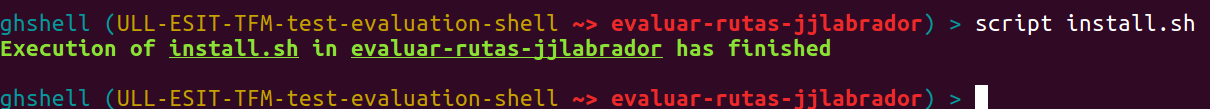
\includegraphics[width=1\textwidth]{images/ghshell7-3}
		\caption{Ejecución del script 'install.sh' en el repositorio actual}
		\label{fig:ghshell7-3}
		\end{center}
		\end{figure}
		
        \begin{figure}[H]
		\begin{center}
		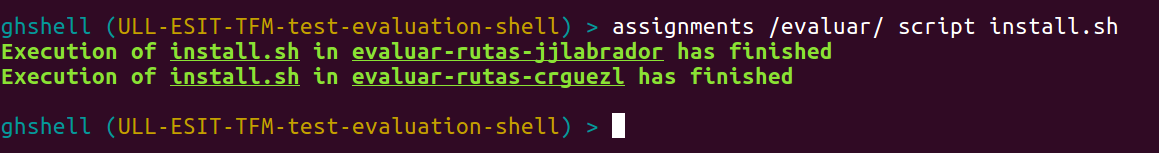
\includegraphics[width=1\textwidth]{images/ghshell7-1}
		\caption{Ejecución del script 'install.sh' en asignaciones que coinciden con una expresión regular}
		\label{fig:ghshell7-1}
		\end{center}
		\end{figure}	
		
		\begin{figure}[H]
		\begin{center}
		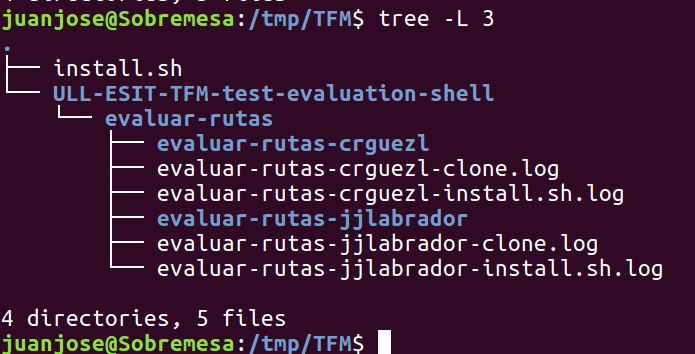
\includegraphics[width=0.7\textwidth]{images/ghshell7-2}
		\caption{Resultado de la ejecución del script 'install.sh'}
		\label{fig:ghshell7-2}
		\end{center}
		\end{figure}
		
%------------------------------------------------------------------------------------------------------------
\subsection{Recopilar la información obtenida de la automatización de tareas}
\label{subsec:3.1.4}

    Una vez ejecutados los scripts necesarios para evaluar un determinado repositorio, es posible generar un {\bfseries GitBook} con el resultado de la ejecución de los mismos. Este libro se genera en formato PDF y en HTML.
\bigskip
    
    En función del contexto dónde nos encontremos dentro de la herramienta, podremos:
    \begin{itemize}
    	\item Crear un GitBook en el repositorio en el que nos encontremos.
    	\item Crear un GitBook en un determinado repositorio.
	    \item Crear un GitBook en todos los repositorios que coincidan con una determinada expresión regular.
	    \item Crear un GitBook en todos los repositorios de una asignación coincidan con una determinada expresión regular.
    \end{itemize}
        
        \begin{figure}[H]
		\begin{center}
		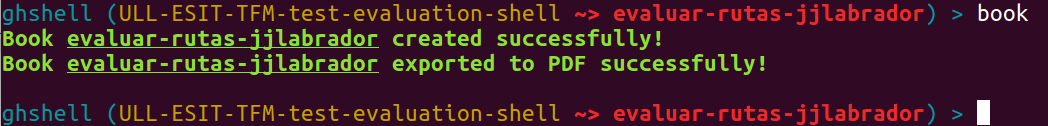
\includegraphics[width=1\textwidth]{images/ghshell8-3}
		\caption{Creación del Gitbook en el repositorio actual}
		\label{fig:ghshell8-3}
		\end{center}
		\end{figure}
		
        \begin{figure}[H]
		\begin{center}
		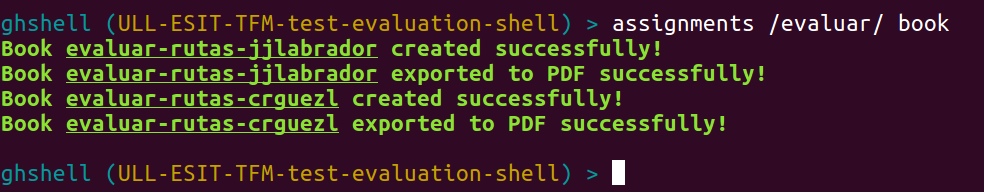
\includegraphics[width=1\textwidth]{images/ghshell8-1}
		\caption{Creación del Gitbook en asignaciones que coinciden con una expresión regular}
		\label{fig:ghshell8-1}
		\end{center}
		\end{figure}	
		
		
		Se puede observar el progreso de la creación del libro revisando los ficheros de logs que se generan: \textless \verb|nombre-repositorio|\textgreater \verb|-gitbook_build.out| y \textless \verb|nombre-repositorio|\textgreater \verb|-gitbook_pdf.out|.
		
\bigskip
		Tanto el PDF como el HTML, contarán con las siguientes páginas:
		
		\begin{itemize}
			\item Índice (Tabla de contenidos).
			\item Introducción: en esta página se copiará el fichero {\it README.md} del repositorio. En caso de que no tuviera ese fichero, se imprimirá un mensaje que indica que el repositorio no tiene fichero README.md.
			\item Páginas correspondientes a la ejecución de cada script.
		\end{itemize}
		
		
		\begin{figure}[H]
		\begin{center}
		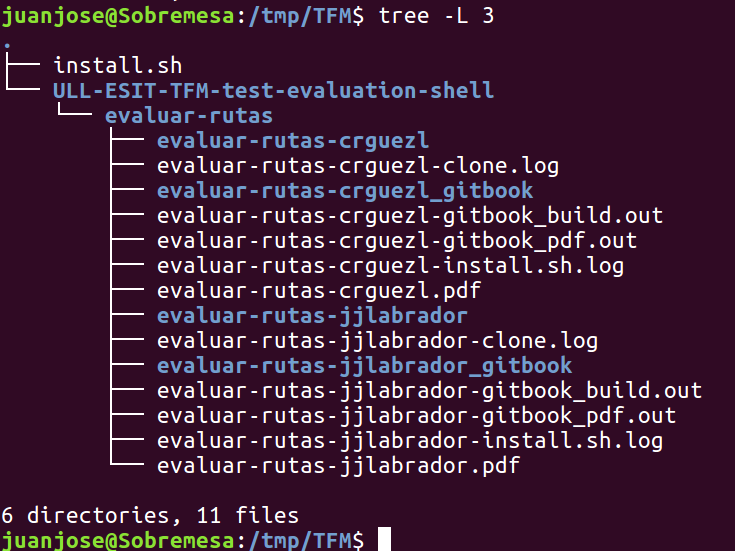
\includegraphics[width=0.7\textwidth]{images/ghshell8-2}
		\caption{Resultado de la creación del Gitbook}
		\label{fig:ghshell8-2}
		\end{center}
		\end{figure}
		
		La carpeta que contiene el libro en HTML se llamará: \newline
		\textless \verb|nombre-repositorio|\textgreater \verb|_gitbook/|\verb|_book|. 
		
		\begin{figure}[H]
		\begin{center}
		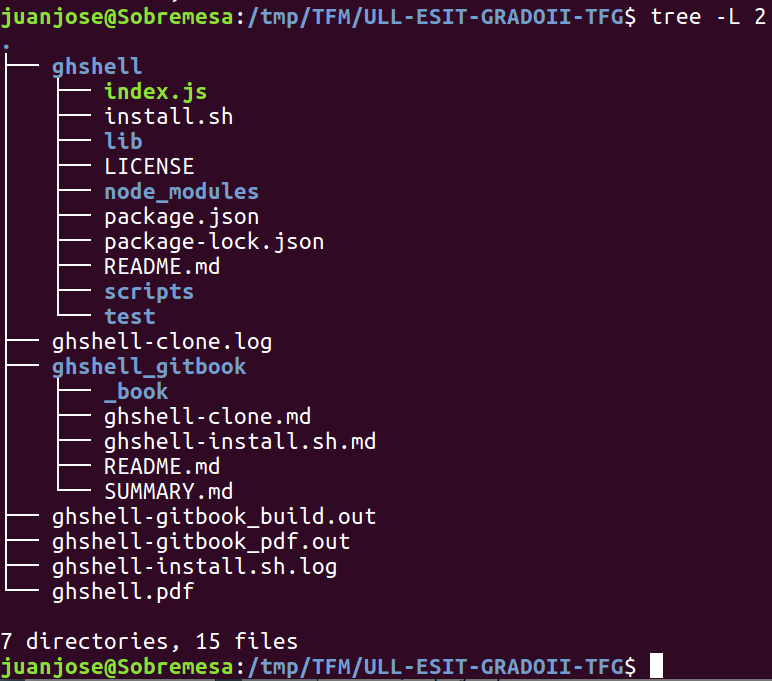
\includegraphics[width=0.7\textwidth]{images/ghshell8-4}
		\caption{Localización del HTML del Gitbook}
		\label{fig:ghshell8-4}
		\end{center}
		\end{figure}
		
		
		El fichero PDF que se genera se llamará \textless \verb|nombre-repositorio|\textgreater \verb|.pdf|. 
        		
        
        \begin{figure}[H]
		\begin{center}
		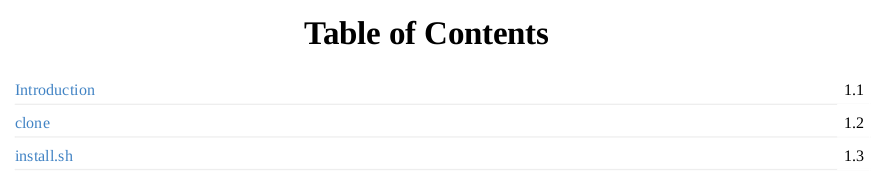
\includegraphics[width=0.9\textwidth]{images/ghshell8-6}
		\caption{Indice del PDF generado}
		\label{fig:ghshell8-6}
		\end{center}
		\end{figure}
		
		\begin{figure}[H]
		\begin{center}
		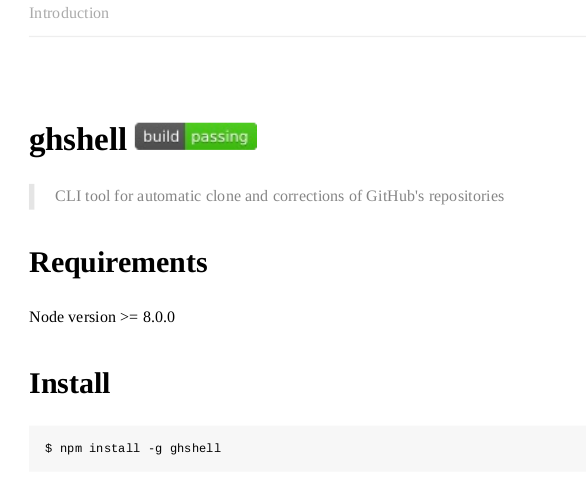
\includegraphics[width=0.7\textwidth]{images/ghshell8-7}
		\caption{Introducción del PDF generado}
		\label{fig:ghshell8-7}
		\end{center}
		\end{figure}
		
		\begin{figure}[H]
		\begin{center}
		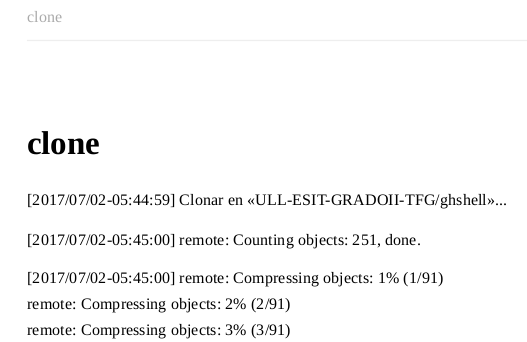
\includegraphics[width=0.7\textwidth]{images/ghshell8-8}
		\caption{Resultado del clonado del repositorio}
		\label{fig:ghshell8-8}
		\end{center}
		\end{figure}
		
		\begin{figure}[H]
		\begin{center}
		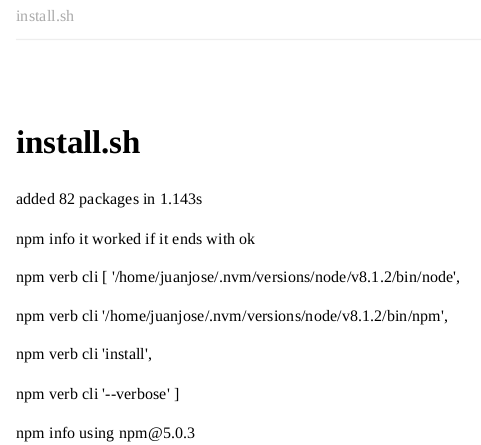
\includegraphics[width=0.7\textwidth]{images/ghshell8-9}
		\caption{Resultado de la ejecución del script en el repositorio}
		\label{fig:ghshell8-9}
		\end{center}
		\end{figure}        		
  		
\newpage
%---------------------------------------------------------------------------------
\section{Funcionalidades extra}
\label{3:sec:2}

Además de las funcionales solicitadas en este Trabajo de Fin de Máster, se han añadido una serie de funcionalidades extra que, a pesar de no ser requeridas, brindan al usuario de una mejor experiencia de uso del programa:

\begin{itemize}
	\item \underline{Autocompletado de los comandos disponibles}, pulsando tabulador, en función del contexto donde nos encontremos (nivel principal, organización o repositorio):
	
		\begin{figure}[H]
		\begin{center}
		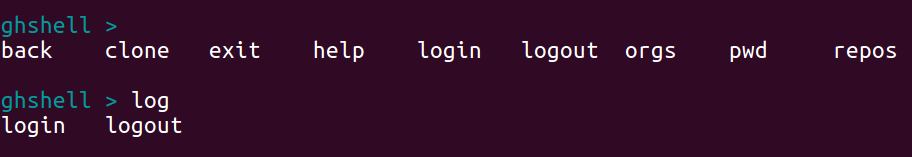
\includegraphics[width=1\textwidth]{images/tab1-1}
		\caption{Autocompletado de comandos}
		\label{fig:tab1-1}
		\end{center}
		\end{figure}
	
	
	Además, también es posible autocompletar los nombres de las organizaciones y repositorios, haciendo mucho más fácil su escritura:
	
		\begin{figure}[H]
		\begin{center}
		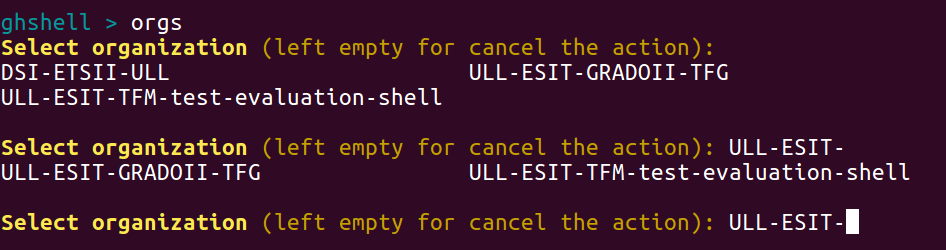
\includegraphics[width=1\textwidth]{images/tab1-2}
		\caption{Autocompletado de organizaciones}
		\label{fig:tab1-1}
		\end{center}
		\end{figure}
		
		\begin{figure}[H]
		\begin{center}
		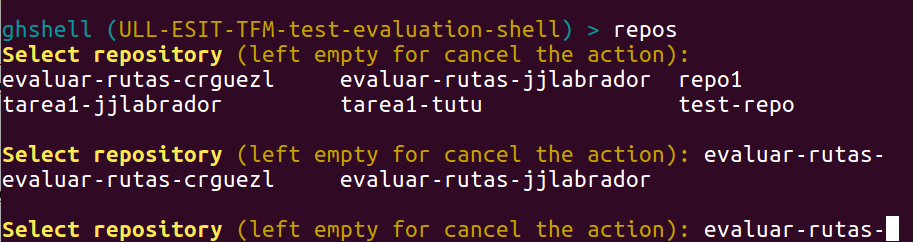
\includegraphics[width=1\textwidth]{images/tab1-3}
		\caption{Autocompletado de repositorios}
		\label{fig:tab1-1}
		\end{center}
		\end{figure}
	
	\item \underline{Opción de ayuda} que muestra la descripción de los comandos y cómo se utilizan. Esta ayuda varía dependiendo del contexto donde nos encontremos:
	
		\begin{figure}[H]
		\begin{center}
		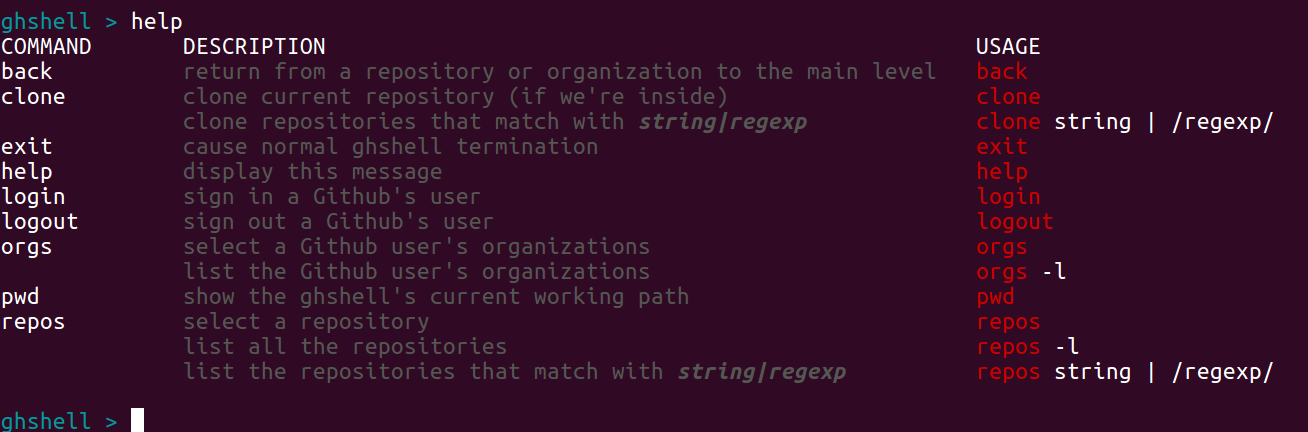
\includegraphics[width=1\textwidth]{images/help1-1}
		\caption{Ayuda global}
		\label{fig:help1-1}
		\end{center}
		\end{figure}
		
		\begin{figure}[H]
		\begin{center}
		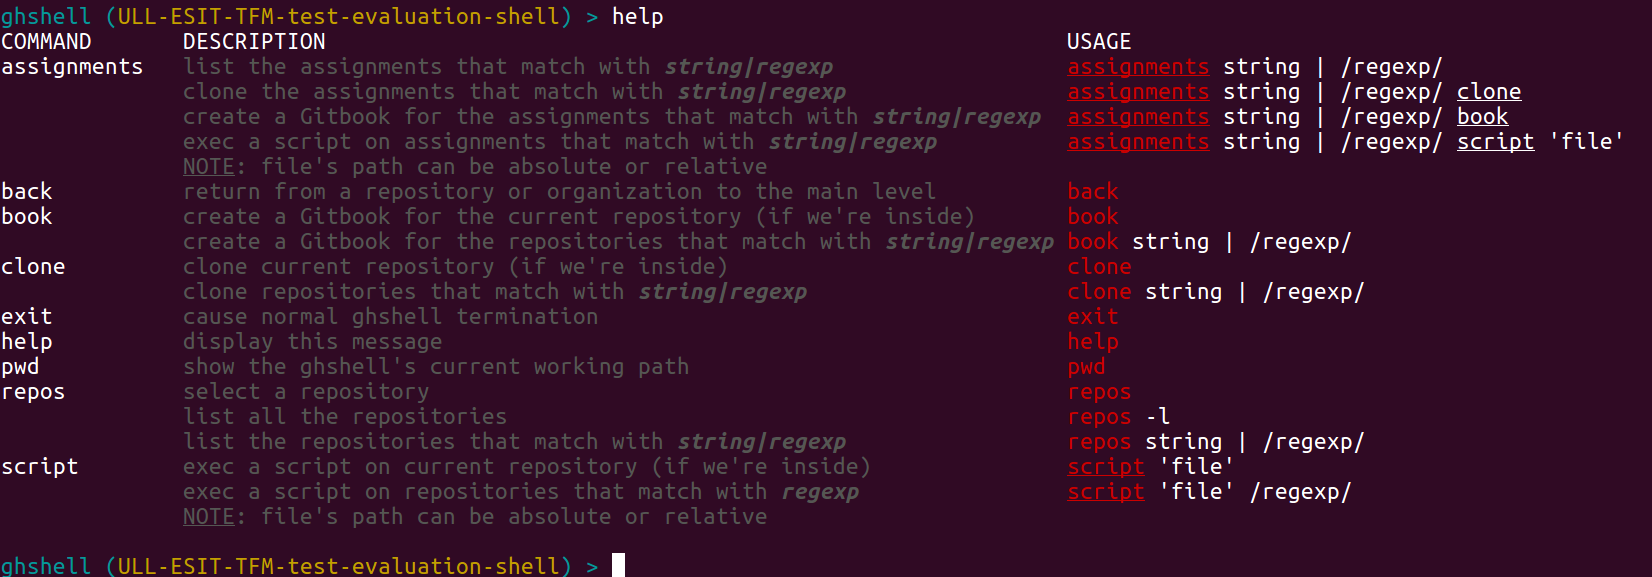
\includegraphics[width=1\textwidth]{images/help1-2}
		\caption{Ayuda en el contexto de organización}
		\label{fig:help1-2}
		\end{center}
		\end{figure}
		
		\begin{figure}[H]
		\begin{center}
		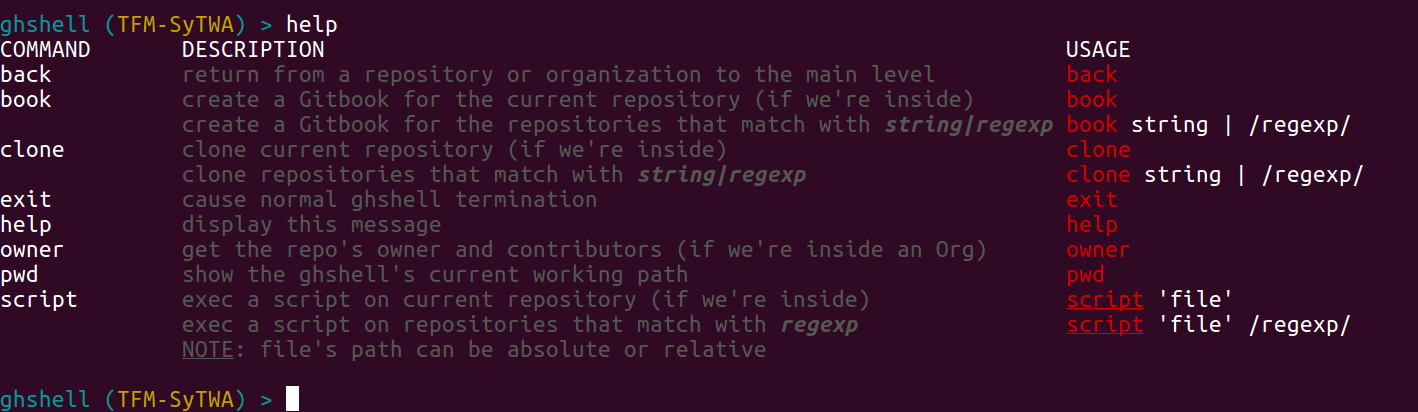
\includegraphics[width=1\textwidth]{images/help1-3}
		\caption{Ayuda en el contexto de repositorio}
		\label{fig:help1-3}
		\end{center}
		\end{figure}
	
	\item \underline{Opción de visualizar el directorio de trabajo actual} (donde se ha ejecutado el programa). Útil para determinar rutas relativas de los scripts que se desean ejecutar.
	
		\begin{figure}[H]
		\begin{center}
		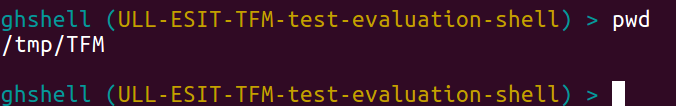
\includegraphics[width=0.7\textwidth]{images/pwd}
		\caption{Directorio actual de trabajo}
		\label{fig:pwd}
		\end{center}
		\end{figure}
	
	
	\item \underline{Opción para conocer el propietario de cada repositorio}. En el caso de que el repositorio pertenezca a una organización, mostrará los contribuyentes de ese repositorio.
\end{itemize}

		\begin{figure}[H]
		\begin{center}
		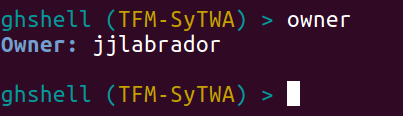
\includegraphics[width=0.5\textwidth]{images/owner1-1}
		\caption{Propietario del repositorio}
		\label{fig:owner1-1}
		\end{center}
		\end{figure}
		
		\begin{figure}[H]
		\begin{center}
		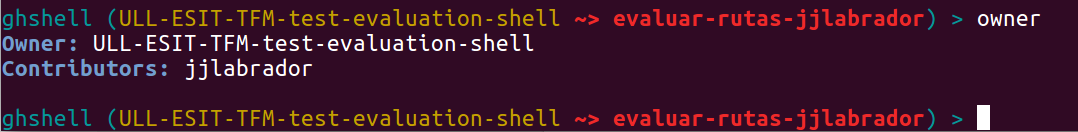
\includegraphics[width=1\textwidth]{images/owner1-2}
		\caption{Contribuyentes del repositorio}
		\label{fig:owner1-2}
		\end{center}
		\end{figure}

\newpage	
%---------------------------------------------------------------------------------
\section{Problemas encontrados y soluciones}
\label{3:sec:3}

A continuación se detallan los problemas encontrados durante la implementación de la herramienta y las soluciones encontradas para los mismos:

%---------------------------------------------------------------------------------
\subsection{Asincronía}
\label{subsec:3.3.1}

Una de las características más importantes del lenguaje \ceis{\ref{apend1:js}} es la asincronía. Usa un modelo de operaciones de entrada/salida sin bloqueo y orientado a eventos, que lo hace ligero y eficiente. Sin embargo, algunas acciones que debía realizar esta herramienta debían de ser síncronas. Ejemplos son el login del usuario y ejecución de scripts.
\bigskip

{\normalsize {\bfseries Solución}}
\bigskip

La solución a este comportamiento pasó por realizar un amplio estudio de la documentación para usar mecanismos que permitieran bloquear la ejecución de la herramienta en las partes que deseábamos. Los mecanismos usados han sido:

\begin{itemize}
	\item \underline{Funciones síncronas del propio lenguaje}.
	\item \ceit{\ref{apend1:promesa}}.
	\item Métodos \ceit{\ref{apend1:async-await}}.
	\item \underline{Librerías} con métodos implementados de manera síncrona.
\end{itemize}

%---------------------------------------------------------------------------------
\subsection{Autocompletado de comandos}
\label{subsec:3.3.2}

Para el manejo de los flujos de lectura y escritura estándar de la herramienta, se ha utilizado la interfaz nativa de Node.js ({\it Readline}). Esta interfaz provee de una función de autocompletado para el texto que escribe el usuario.
\bigskip

Sin embargo, sólo funciona con la primera palabra (comando) que escribe. 
\bigskip

Tras investigar al respecto y buscar posibles librerías alternativas, no existía ninguna solución que corrigiera este comportamiento.
\bigskip

{\normalsize {\bfseries Solución}}
\bigskip

Realizando numerosas pruebas, se halló una manera propia de conseguir completar más de un comando en la misma línea. Cuando realice los test de aceptación pertinentes requeridos por la comunidad de Node, solicitaré un {\bfseries Pull Request} a su repositorio con esta mejora.


%---------------------------------------------------------------------------------
\section{Perfil del usuario de ghshell}
\label{3:sec:4}

El uso de \verb|ghshell| está especialmente dirigido a un determinado grupo de profesores: nos referimos al perfil de un profesor, principalmente docente en alguna rama de Ingeniería, con conocimientos avanzados en programación y en herramientas de control de versiones.
\bigskip

No obstante, ya que la curva de aprendizaje de \verb|ghshell| no es excesiva y dado que el uso de las herramientas de control de versiones no se limita exclusivamente a repositorios de código fuente, se puede extender su uso para el resto de profesorado y usuarios con otros roles. Basta con tener claras unas nociones básicas de informática, junto con la lectura y asimilación previa de la documentación de la herramienta.
